\documentclass{article}
\usepackage[margin=0.75in]{geometry}
\usepackage{graphicx} 
\usepackage{natbib} 
\usepackage{amsmath} 
\setlength\parindent{0pt} % Removes all indentation from paragraphs
\addtolength{\topmargin}{-0.40in}
\usepackage[parfill]{parskip}
\usepackage{datetime}
\usepackage{fancyhdr}
\pagestyle{fancyplain}
\fancyhead{}
\fancyfoot[L]{}
\fancyfoot[C]{FSAA 2020 Laboratory 1}
\fancyfoot[R]{\thepage}
%\usepackage{times} % Uncomment to use the Times New Roman font

%----------------------------------------------------------------------------------------
%	DOCUMENT INFORMATION
%----------------------------------------------------------------------------------------

\title{Laboratory 1 : Build a Simple Bank}
%\author{Jacky Mallett}

\begin{document}
\newdate{date}{27}{04}{2020}
\date{\displaydate{date}}
\maketitle % Insert the title, author and date

% If you wish to include an abstract, uncomment the lines below
% \begin{abstract}
% Abstract text
% \end{abstract}

%----------------------------------------------------------------------------------------
%	SECTION 1
%----------------------------------------------------------------------------------------

\section*{\centering Objectives}
Familiarity with Threadneedle, fractional reserve banking operations and
cental bank reserve regulation.

\subsection*{Tips}
The Save and Load buttons save and load the current configuration respectively. Judiciously
saving the configuration once created will allow it to be re-run repeatedly by re-loading.
\par
Reset will remove all agents from the simulation.

% If you have more than one objective, uncomment the below:
%\begin{description}
%\item[First Objective] \hfill \\
%Objective 1 text
%\item[Second Objective] \hfill \\
%Objective 2 text
%\end{description}

%\subsection{Definitions}
%\label{definitions}
%\begin{description}
%\item[Stoichiometry]
%The relationship between the relative quantities of substances taking part in a reaction or forming a compound, typically a ratio of whole integers.
%\item[Atomic mass]
%The mass of an atom of a chemical element expressed in atomic mass units. It is approximately equivalent to the number of protons and neutrons in the atom (the mass number) or to the average number allowing for the relative abundances of different isotopes. 
%\end{description} 
 
%----------------------------------------------------------------------------------------
%	SECTION 2
%----------------------------------------------------------------------------------------

\section{Create a Bank}
\begin{figure}[h]
\begin{center}
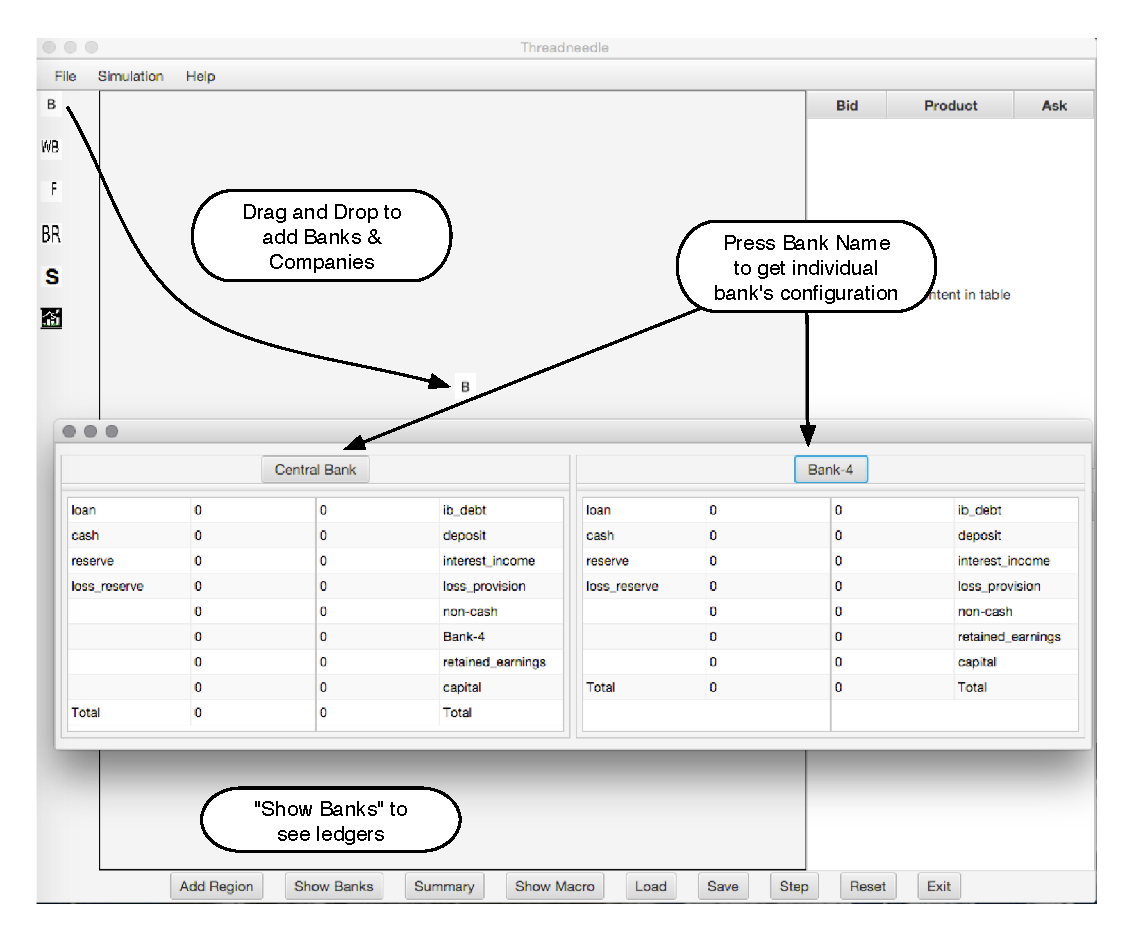
\includegraphics[width=12cm]{lab_fig_1.eps} 
\caption{Create Bank and Bring up Ledger}
\end{center}
\end{figure}

\begin{enumerate}
\item Drag and drop a Bank from the left hand side menu onto the main screen.
\item Use the "Show Banks" button to bring up the Bank balance display.
\end{enumerate}

\section{Setup Bank Cash and Capital}
\subsection*{Tip}
Holding the mouse pointer over a field will bring up a tool tip to explain it.
\begin{figure}[h]
\begin{center}
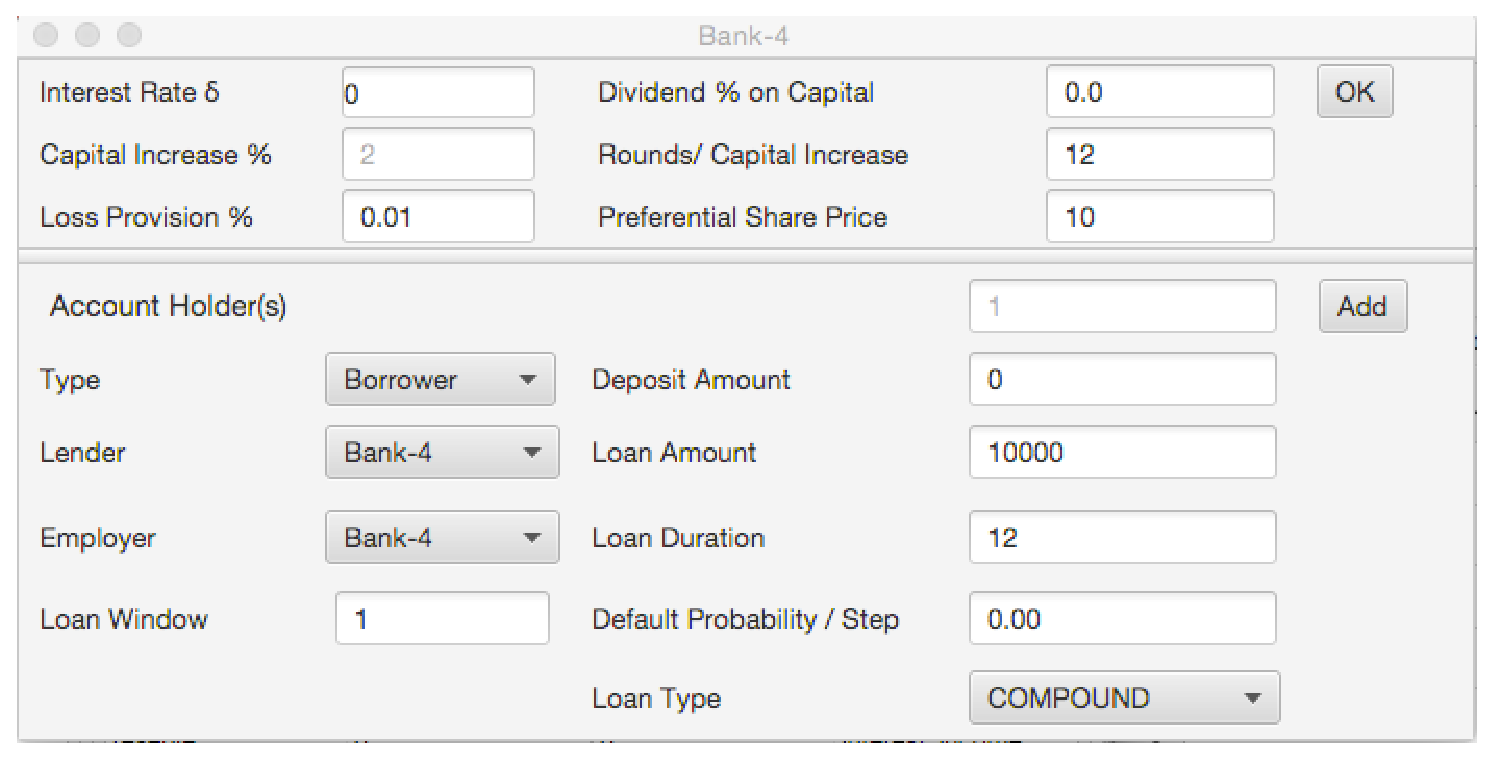
\includegraphics[width=12cm]{lab_fig_2.eps} 
\caption{Bank Configuration}
\end{center}
\end{figure}
Pressing on the Bank's name in the ledger screen will bring up an 
individual configuration menu for the bank. This screen can be
used to set interest rates for the Bank, and also to add account holders
with specific, bank related, behaviours.
\par
There are three such agents, Borrowers, Savers and Investors. Borrowers take out
loans from Banks and receive a salary from the bank to repay them. Investors
provide purchase capital from the bank, and may receive dividend income on that
capital, savers simply deposit money (cash).

\begin{enumerate}
\item Bring up the central bank menu, and set regulation to be reserve
only.
\item Add a single borrower, with a 12 month loan, for 10,000 and a 1,000
initial deposit.
\item Step the simulation forward 10 steps. Note: each step is one day,
but if you rotate the step button it will provide
a bigger increment.
\item What happens?
\item What is the correct reserve requirement for a loan of 10,000 with
1,000 in asset cash?
\item Add a saver with the additional amount as a deposit and step forward
200 steps. Why is the observed behaviour cyclical?
\end{enumerate}

\section{Expansion from Initial Conditions}
\begin{enumerate}
\item Set central bank regulation to be reserve only.
\item Pick a reserve rate of your choice.
\item Estimate the total expansion of deposits for the current configuration.
\item Run the simulation and explain the results.
\item The central bank increases interest rates by 2\%. What do you expect to happen?
\item What does happen? Why?
\end{enumerate}

\section{Expansion 2}
Explore what combinations of initial deposits, borrowers, loans and interest rates 
will maximise expansion under reserve requirement regulation?

Using such a simulation, run the simulation until it hits the reserve limit. 
Now add another loan/borrower combination with a default probability of 50\%.

What happens?
\section*{Notes}
In reality, gold standard reserve regulated banks would maintain minimum
capital holdings, as well as their regulatory required reserve holdings.
Bank Capital is a fairly general term and is used to cover a number of
ledger items including loss reserves, retained income, and the 
preferential shares issued by banks in exchange for the cash deposits 
provided by their Investors.
%\par
%Book keeping and accounting treatments have also changed over time. For
%example, this balance ledger is from the Australian Banking System, 
%circa...


\end{document}
